\documentclass{article}
\usepackage{amsmath}
\usepackage{graphicx}
\usepackage{setspace}
\usepackage[affil-it]{authblk}
\usepackage[left=3cm, right=3cm, top=3cm, bottom=3cm]{geometry}
\usepackage{multicol}
\usepackage{listings}
\usepackage[linesnumbered,ruled,vlined]{algorithm2e}
\usepackage{algpseudocode,amsthm}
\usepackage{calrsfs}
\DeclareMathAlphabet{\pazocal}{OMS}{zplm}{m}{n}
\usepackage[hidelinks]{hyperref}

\title{CS513: Analysis of Randomized Search Tree (Treap)}
\date{}
\author{Prateekshya Priyadarshini}
\affil{M.Tech CSE}
\setcounter{tocdepth}{3}
\begin{document}
\tableofcontents
\newpage
\pagenumbering{arabic}
\maketitle

\section{Introduction to Randomized Search Tree (Treap)}
Randomized Search Tree (Treap) is a data structure which combines heap and tree properties. The nodes of treap contain both key and priority. The keys follow the properties of a binary search tree and the priorities follow the properties of a heap. A sample treap is shown below. The numbers within the bracket present the priority. In this document, we use treap and randomized search tree interchangeably.
\begin{center}
\includegraphics[scale=0.3]{SampleTreap.png}
\end{center}

\subsection{Insertion}
\label{insert}
In case of insertion, we traverse the tree from root towards the leaf by following the property of binary search tree and attach the new node at its right position. Then we check for the heap property. If the priority of the newly inserted node is less than the priority of its parent, then we do a single rotation after which the child becomes the parent and vice versa. This process of checking and rotation will go up till root or till the point where we don't get such inversion condition. The worst case time complexity is $O(n)$ and average case time complexity is $O(\log n)$.\newline
\begin{center}
\includegraphics[scale=0.5]{BeforeInsert.png}
\end{center}
After inserting 246-
\begin{center}
\includegraphics[scale=0.5]{AfterInsert.png}
\end{center}

\subsection{Deletion}
\label{delete}
To delete a node, we first search it. Then we keep rotating till the node to be deleted becomes a leaf node and the node is then detached from the tree. When the node has two children, we rotate by holding the child having less priority. This ensures the maintenance of heap property. The worst case time complexity is $O(n)$ and average case time complexity is $O(\log n)$.
\begin{center}
\includegraphics[scale=0.5]{BeforeDelete.png}
\end{center}
After deleting 149-
\begin{center}
\includegraphics[scale=0.5]{AfterDelete.png}
\end{center}

\subsection{Searching}
\label{search}
Searching process is similar to that of binary search tree. The worst case time complexity is $O(n)$ and average case time complexity is $O(\log n)$.



\section{Related Work}
\subsection{General Approaches}
\subsubsection{Keeping a dummy node to hold the tree}
For making rotation easier, one dummy node is taken. The actual tree is stored at the right child of the dummy node. It makes rotation easier when the root itself is imbalanced.
\subsubsection{Using level order traversal for printing the tree}
Since the order of nodes mentioned in the graphviz file is important, we need to do a traversal of the tree starting from the root such that the root should be mentioned at the top. This can be done using either preorder traversal or level order traversal. Here level order traversal is being considered and a separate queue is implemented for that purpose.
\subsubsection{Two global variables for printing the tree}
\begin{enumerate}
	\item \textbf{fileCount}\newline
	This variable is initialized to 0. It gets incremented everytime a new graphviz file is created. So that we can create different files each time. For example-graph0.gv,graph1.gv,graph2.gv etc.
	\item \textbf{fileType}\newline
	This variable stores 0 for windows OS, 1 for linux OS. More options can be added as per requirement. This variable helps us to decide which type of commands file we have to create. If we are in windows, we need to add all the commands needed to convert graphviz files to png files into a batch file. Similary in linux we have to add all of them to a shell script.
\end{enumerate}
\subsubsection{Creating batch files or shell scripts}
Since the commands to generate a .png file from a .gv file are not straight forward for a beginner, this program generates batch file in windows and shell script in linux which contains all those commands. Every time a new tree is printed, these files get executed and the respective images get generated. For reference, the images won't be deleted or replaced till the program is being executed.
\subsubsection{Storing the entire execution process}
The entire execution process is stored in \textbf{$<user\_given\_name>$output.txt}. This file can be referred to check what went wrong, which images refer to which trees etc. Also the graphviz files and png files are stored along with a sequence number i.e. \textbf{$<user\_given\_name>$1.png} or \textbf{$<user\_given\_name>$9.gv}.
\subsubsection{Commands used for various operations}
\textbf{For makefile}
\begin{enumerate}
	\item g++ -c TreapImpl.cpp
	\item g++ -o TreapImpl TreapImpl.o
\end{enumerate}
\textbf{For valgrind}
\begin{enumerate}
	\item g++ -o TreapImpl -g TreapImpl.cpp
	\item valgrind --tool=memcheck --leak-check=yes --show-reachable=yes --num-callers=20 --track-fds=yes ./TreapImpl
\end{enumerate}
\subsubsection{Header files for making the code modularized}
There are three header files i.e. nodes.h (contains all the node structures), datastructures.h (contains all the class definitions) and functions.h (contains all the function definitions).
\subsection{Approaches taking Performance Evaluation into consideration}
\subsubsection{One hybrid code for all types of testing}
The same code of treap can be used for testing treap operations as well as comparing the performance with binary search tree and AVL tree. Also, multiple input files can be given one after another till quit is hit. For example- if someone wants to run only treap with manual input file, then he/she has to create an input file in the mentioned format and give the name. If the performances are to be compared, then random input files can be generated. A mix of manual input files and randomly generated input files can also be given. These things can be chosen in the runtime itself.
\subsubsection{Progress bar for larger input files}
A progress bar starts appearing if the input file size is larger than 1000 i.e. if the total number of operations is more than 1000. It makes things easier since we can trace how much time the execution is going to take for larger input files of size a million or a few millions. Progress bar appears only for randomly generated input files. Keep the width of the console window large enough to view a proper progress bar.
\subsubsection{Ratio input by user}
Insertion to deletion ratio should be given at the run time. If random ratio is the requirement, then the input should be $0$ at that place. e.g. If the input is $70$, it will perform around $70\%$ insertions and around $30\%$ deletions. But, if the input is $0$, the random ratio generator supports at least $55\%$ insertions and at most $85\%$ insertions. So, it will generate a random number between $55-85$.
\subsubsection{Smaller Range for running experiments}
For comparison purpose, the range of random numbers was at most $32767$ i.e. $RAND\_MAX$. But, the test case generation function supports random number generation upto $2147483767$ i.e. $INT\_MAX$. The default $rand()$ supports random number upto $RAND\_MAX$. Hence, here $(rand()*rand()*2)-1$ is done to increase the range upto $INT\_MAX$ because $rand()*rand()*2 = INT\_MAX+1$. Sample evaluation files for huge trees (e.g. $60,00,000$ nodes) are also attached. 
\subsubsection{Semi-merging files for three different programs}
If the code execution breaks while executing BST or AVL tree (may be due to power failure or insufficient storage allocation), it is cumbersome to restart the entire process starting from treap for larger number of operations (i.e. a few millions). So, BST and AVL tree programs are not added as header files. Rather, all are different cpp files in different folders. A batch file or shell script is being generated to carry out the automated execution. Now if the code breaks during AVL tree execution, you can just execute the avlt.cpp file inside the AVLT directory with 3 command line arguments, since treap and BST executions are already complete. For command line argument description, check \ref{instn}, point-19.
\subsection{Parameters chosen for Evaluation}
\begin{itemize}
	\item Total number of insertion and deletion operations
	\item Total number of key comparisons during insertion and deletion
	\item Total number of rotations during insertion and deletion
	\item Height of the tree
	\item Average height of the nodes from root
	\item Average height of the nodes from leaf nodes
	\item Total number of nodes in the final tree
\end{itemize}



\section{Flow of Execution}
\subsection{Random testcase generation: Logic and Procedure}
\subsubsection{Logic}
\begin{itemize}
	\item \textbf{Storing inserted elements in an array}\newline
	So, for keeping track of the elements inserted, there is an array of size $200,000$ which will store the inserted elements one by one in a circular fashion in the first $100,000$ positions. That means once the first half of the array is full, it will start storing from $0^{th}$ index again. The second half of the array will contain random numbers not guaranteed to be in the tree. This will ensure a good mix of present and absent nodes deletion.
	\item \textbf{A few compulsory insertions initially}\newline
	Initially, we do $10\%$ of the total operations or $20$ insertions, whichever is smalller. For example- For $100$ operations, $10$ initial insertions will be there, but for $1000$ operations there will be $20$ initial insertions. Due to this reason, we're getting a slightly greater number of insertions than the ratio given, which is still acceptable for larger number of operations.
	\item \textbf{Choosing an operation}\newline
	During runtime, user gives a number from $1$ to $100$ which will be the ratio of insertion and deletion. If the user gives $0$ then a random value is generated on behalf of the user. For example- if the ratio value is $65$, it means $65\%$ of the operations will be insertions and the rest will be deletions. Since, we usually have more insertions than deletions, the random ratio generator generates numbers between $55$ to $85$. But, the user can give any number in $1-100$ range. After getting this value, for each operation we keep generating random numbers in $1-100$ range. If this value is less than or equal to the ratio, we go for insertion, otherwise we go for deletion.
	\item \textbf{Insertion}\newline
	A random number within the given range is being generated. "insert number" is being written to the input file. If the number is not already generated, then it gets stored to the array.
	\item \textbf{Deletion}\newline
	For, deletion a random index of the array is being generated. For example- if there are $100$ elements in the array, the random index generator will generate a random number in $1-125$ range. Extra $25\%$ is to ensure a mix of present and absent elements. This percentage can be changed in the code. After generating the index, the corresponding element in the array is being selected and "delete number" is being written to the input file.
	\item \textbf{Intermediate Print}\newline
	During runtime, if the user chooses to print the tree images, a few intermediate print commands is being added. The number of print commands is around $10\%$ of the total number of operations. The first intermediate print command is being added after the initial compulsory insertions. Afterwards, if we have a continuous run of insertions, print command is not being added, but it sets a flag to true indicating that we are not adding print commands. Only when we go to delete block, it checks if the flag is true, it sets flag to false. Then it checks if the last $5$ commands are not print commands, then it adds a print command.
	\item \textbf{Footnote}\newline
	This program can run for a billion operations as well (data type can be changed from integer to double and a trillion operations can also be performed. Prerequisite: A hard disk with a few TB capacity).
\end{itemize}
\subsubsection{What user has to do}
User has to give proper inputs carefully during run time. The ratio value should not exceed the range of $1-100$. The range of key values and the number of operations should not exceed the range of integer supported by $C++$. 

\subsection{Manual testcase generation}
insert 9\newline
insert 10\newline
insert 5\newline
delete 6\newline
delete 10\newline
insert 7\newline
search 7\newline
print\newline
delete 10\newline
print\newline
quit\newline\newline
The above sequence can be written as a test case into a file. The same file name can be given in the console during runtime.
\subsection{User prompt}
After executing the program,a prompt will ask the user to enter a number indicating the current operating system followed by the file name. Then it asks for the range of the elements of the treap. The input to this can be an integer only. Similarly it will ask for the percentage of insertion operations. Then it asks whether the user wants to give a manual input file or generate a random file. If manual input file is chosen, then a .txt file should be created in the given format and the name should be given on the console . If random input file generation is chosen, it will further ask for the number of operations. If the number is larger than 1000, it will ask whether intermediate print ocmmands will be added or not. If the input to this is "N" or "n", then only one .gv file will be created at the end. Also the image generation decision is upto the user. Then the user has to enter whether he/she wants to give further input files or wants to stop right after the current input file. Accrodingly quit command will be added at the end.\newline
After all the input files are processed, the prompt will ask whether the user wants to do performance comparison and accordingly further executions will happen. A complete sample prompt is attached below.
\begin{center}
\includegraphics[scale=0.6]{SamplePrompt1.png}
\end{center}
\begin{center}
\includegraphics[scale=0.6]{SamplePrompt2.png}
\end{center}
\begin{center}
\includegraphics[scale=0.6]{SamplePrompt3.png}
\end{center}

\subsection{Instructions to execute the code}
\label{instn}
\begin{enumerate}
	\item If you're using Dev C++, Follow the steps to support $unordered\_map$. Go to tools--compiler option--general tab--tick mark option (add the following commands when calling compiler)--add -std=c++11 there. Then build and execute the project.
	\item In linux or GNU windows compiler, open the terminal or command prompt and type "g++ TreapImpl.cpp" and hit enter.
	\item Then for linux type "./a.out". For windows type "a.exe" or "TreapImpl.exe" (One of them should work). Hit enter.
	\item You can also write "./TreapImpl" and hit enter to execute the makefile which is provided.
	\item Now the prompt will be displayed. Enter 0 or 1 for windows or linux respectively.
	\item Give a name for all the files which are going to be generated during execution.
	\item Write a .txt file according to the given format and enter the file name there. If you give wrong sequence, it can destroy the execution. Alternatively you can choose random file generation.
	\item You can write "quit" or "view" instead of file name to exit from the program or to generate the images till now respectively. However, adding a quit command at the end of the input file is suggested.
	\item The entire execution process can be visualized in $<user\_given\_name>Output.txt$.
	\item The performance comparison of the current execution can be visualized in $evaluation.txt$.
	\item After printing a tree, you can view the images in the same directory. The respective file names are written in the output file.
	\item You can give multiple .txt files one after another. For example- in the first run, you can insert a few nodes and delete one of them to check how the tree rotates, and after seeing the result you can write another .txt file to delete the root node.
	\item You can run the batch file or shell script to manually generate the images.
	\item A separate batch file or shell script is being generated for performance comparison and the entire process is automated. You need not perform it manually.
	\item Avoid printing images for larger input files (if you choose to print, around $10\%$ of the total operations will be print commands in case of random input files. That means if the number of operations is 100, you can observe 107-110 operations in the input file out of which 7-10 are print commands at various places). One print command is always being added at the end to observe the final tree.
	\item Sometimes the process pauses if you click somewhere in the console. Try pressing some key from the keyboard to continue.
	\item Keep the width of the console window large enough to view a proper progress bar.
	\item If you're using test files having different conventions and you're unable to quit the execution, simply enter $1$ to enter a manual input file and then type "quit" in place of file name.
	\item For executing bst.cpp or avlt.cpp separately (after executing treap at least once), you need 3 command line arguments. First one is the type of OS (0 for Windows and 1 for Linux), second one is the user given file name and third one is the output file name. A sample command for windows can be - a.exe 0 demo demoOutput.txt.
\end{enumerate}



\section{Performance Evaluation: Comparison with Binary Search Tree and AVL Tree}
\subsection{Stability throughout multiple experiments}
For evaluation, the insesrtion:deletion ratios considered were $60:40,65:35,70:30,75:25$ and $80:20$. The number of operations considered were $100,1000,10000,100000$ and $1000000$. Two types of executions were done i.e. all the operations at once and breaking them into three parts of $2:5:3$ operations. For each combination, $10$ experiments were done. The results for $10000$ operations are as follows.\newline
\begin{center}
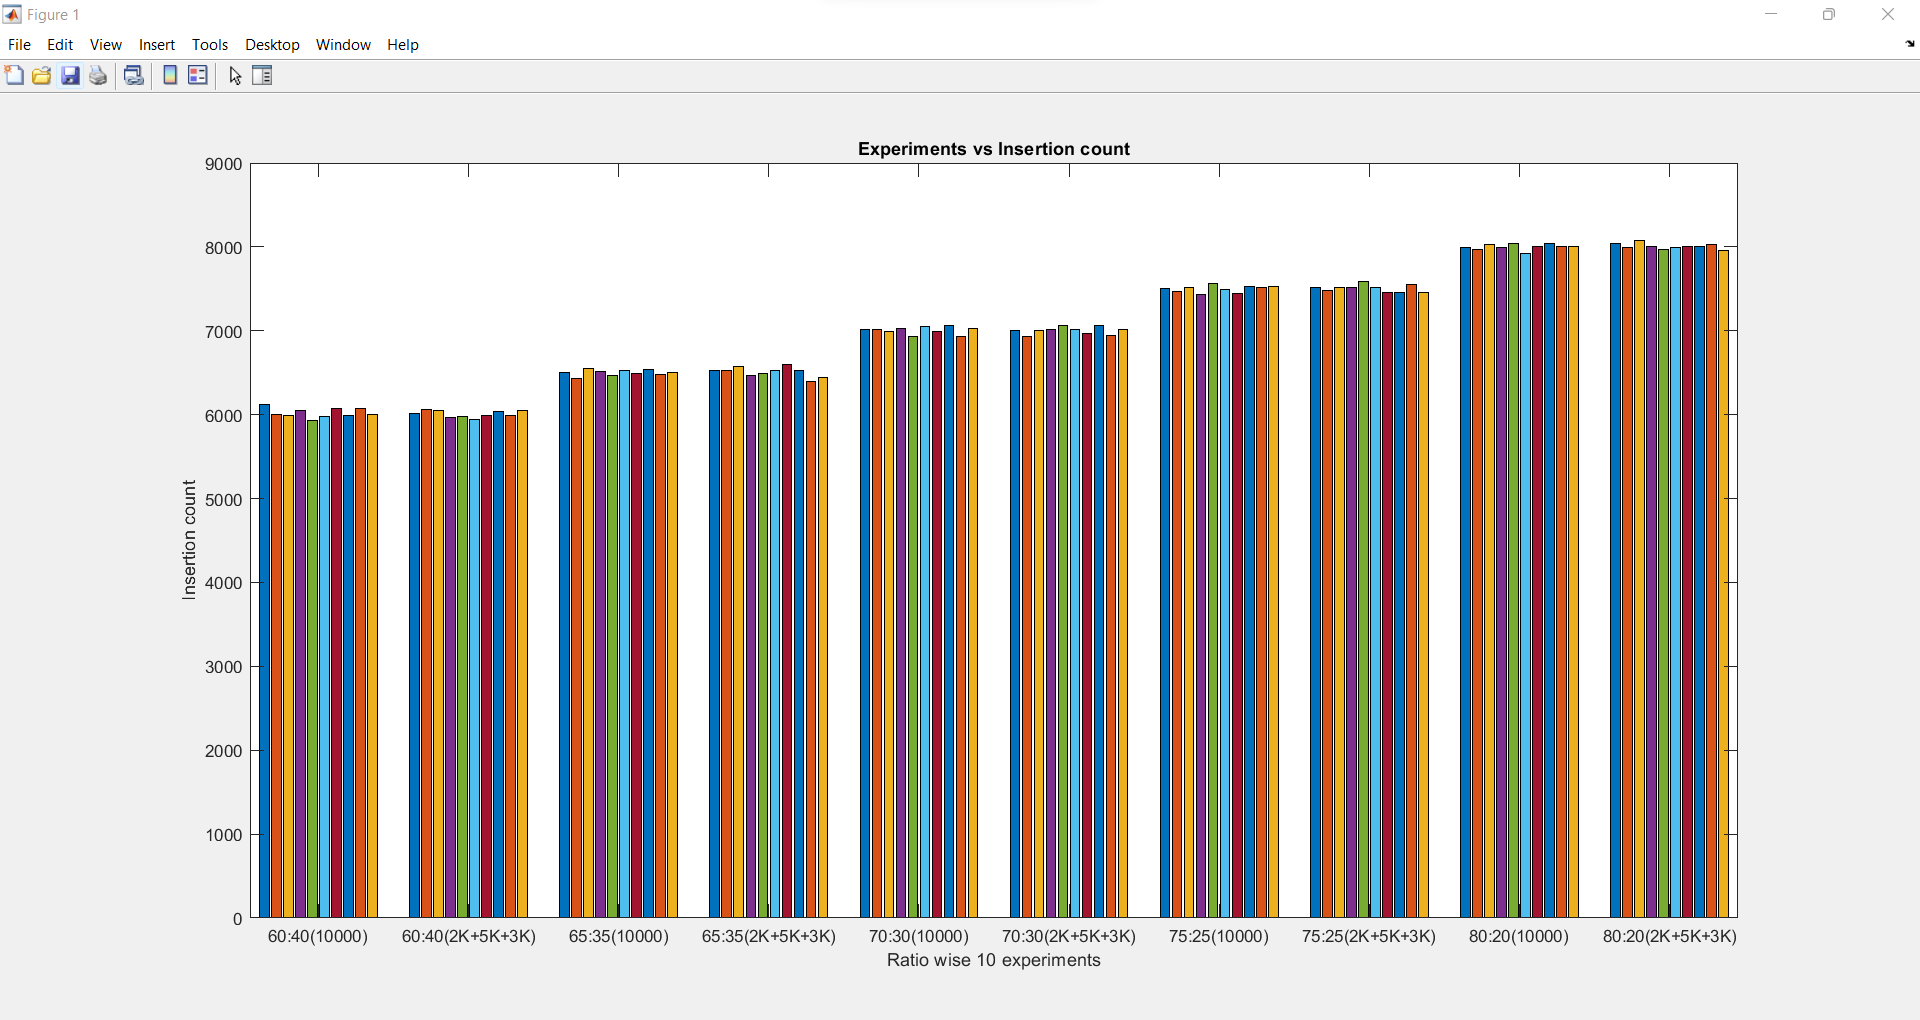
\includegraphics[scale=0.4]{insert.png}
\end{center}
Figure: Total number of insertion operations across multiple executions\newline\newline
This graph plots the total number of insert operations for each ratio with two types of execution (i.e. all the operations at once and breaking them into three parts of $2:5:3$ operations). We can see, for any type of ratio and input combination, the results of $10$ experiments are almost similar. Total number of deletion operations and total number of nodes in the final tree are also similar as follows.
\begin{center}
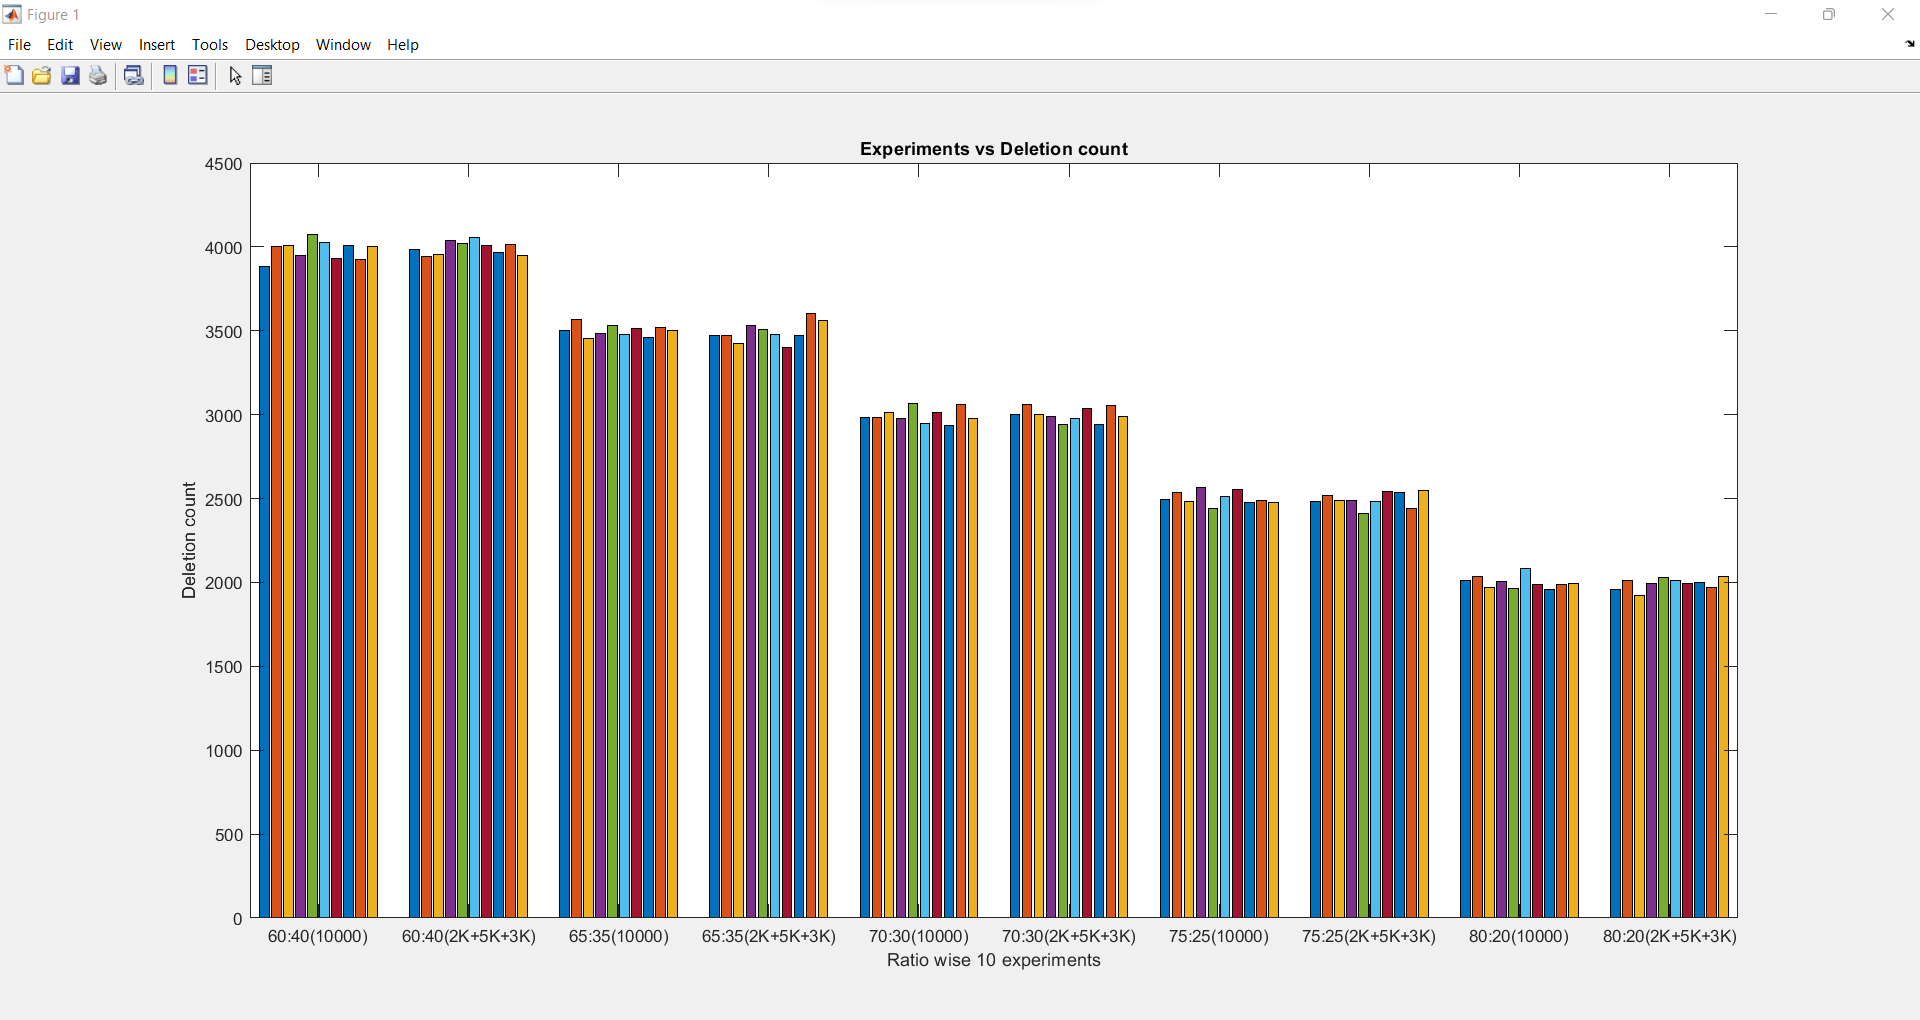
\includegraphics[scale=0.4]{delete.png}
\end{center}
Figure: Total number of deletion operations across multiple executions
\begin{center}
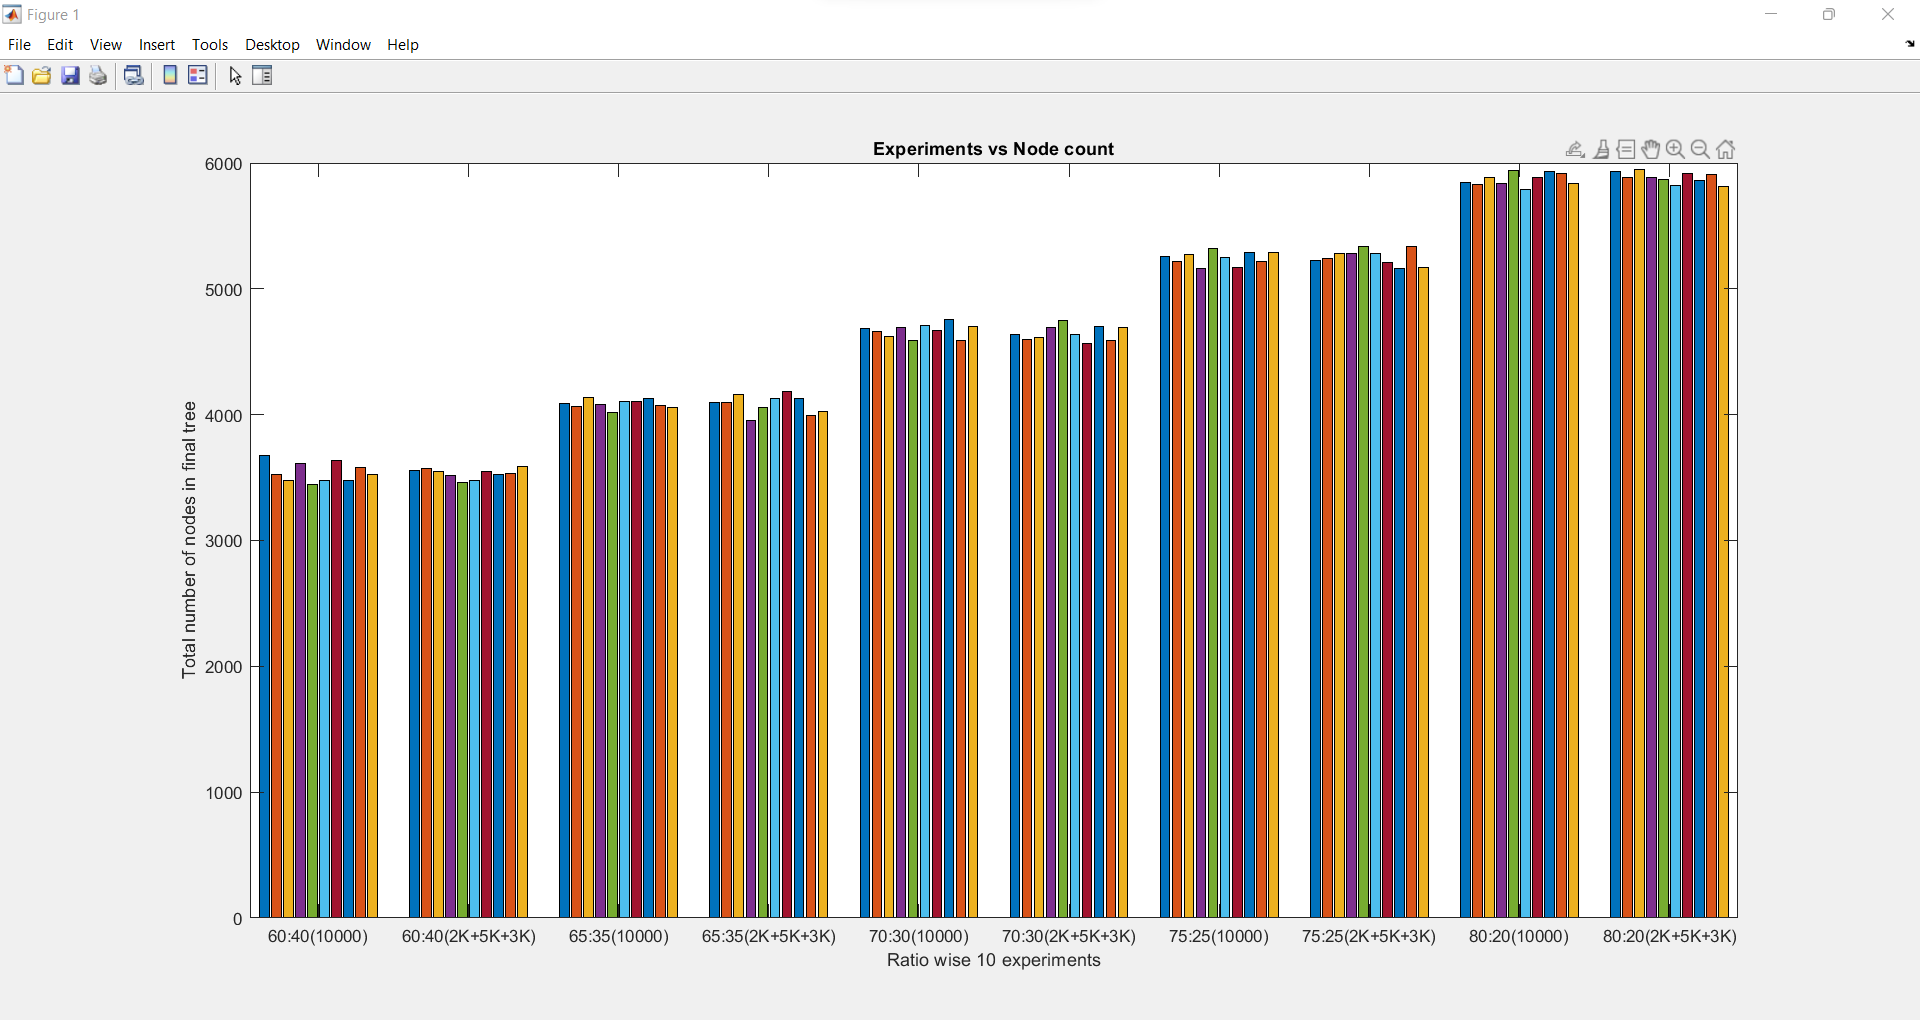
\includegraphics[scale=0.4]{nodecount.png}
\end{center}
Figure: Total number of nodes in the final tree across multiple executions\newline\newline
Hence, we can consider any arbitary experiment and still get similar outcomes.

\subsection{Performance Comparison}
For comparison purpose, the number of operations start from as low as $100$ and go upto as high as a million. All the results are attached below.
\subsubsection{Key Comparisons}
\begin{center}
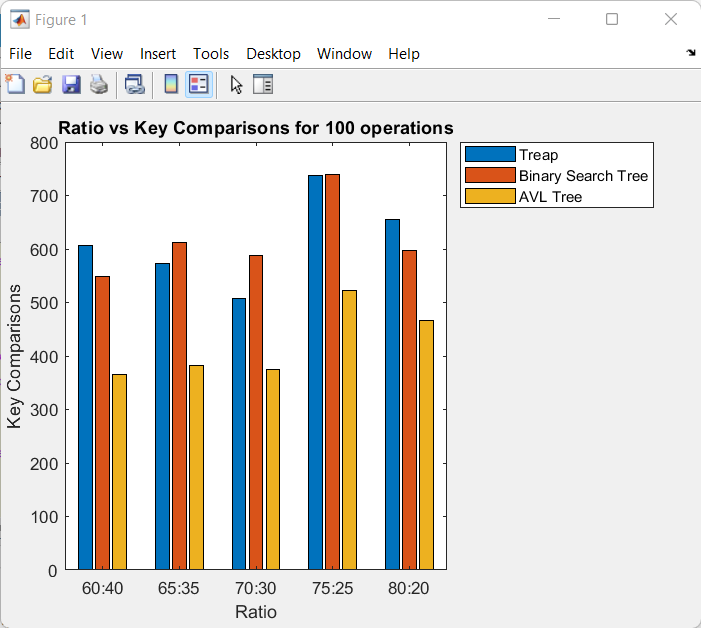
\includegraphics[scale=0.3]{key100.png}
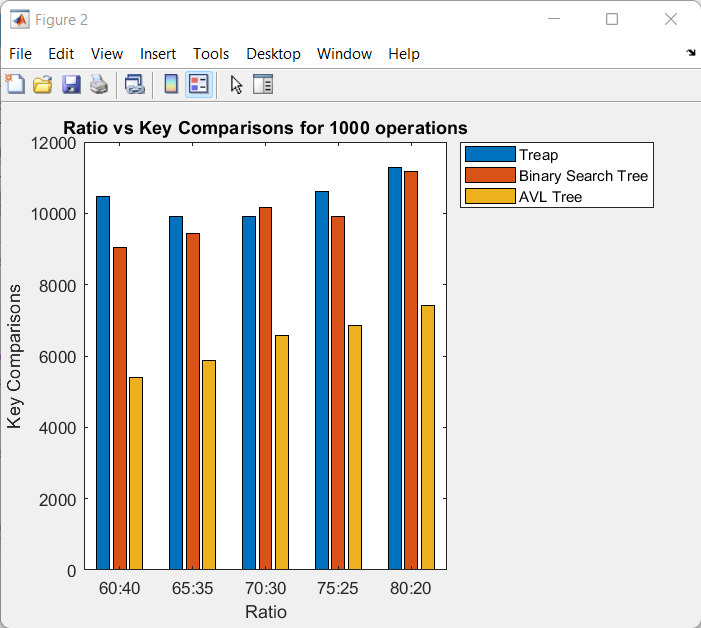
\includegraphics[scale=0.3]{key1K.png}
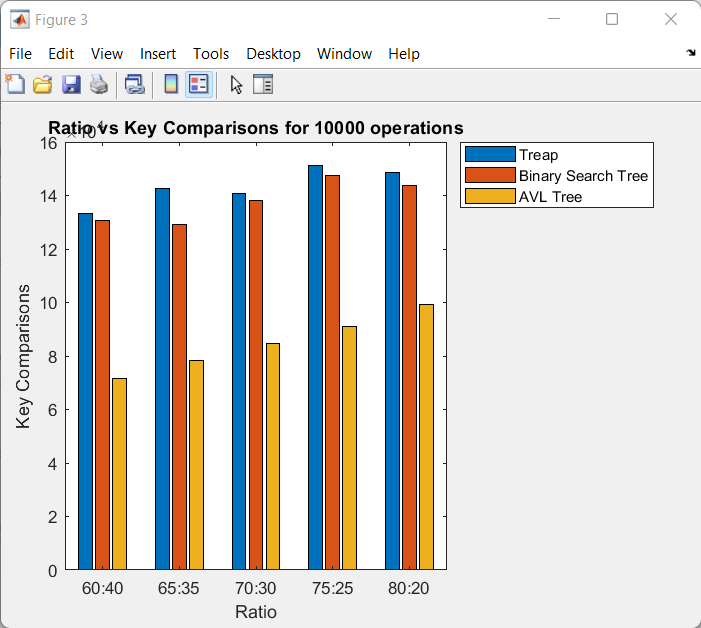
\includegraphics[scale=0.3]{key10K.png}
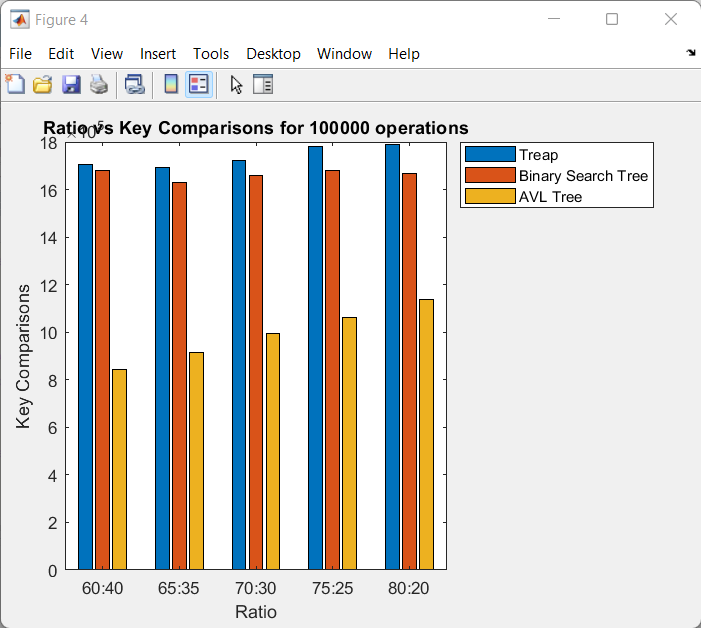
\includegraphics[scale=0.3]{key1L.png}
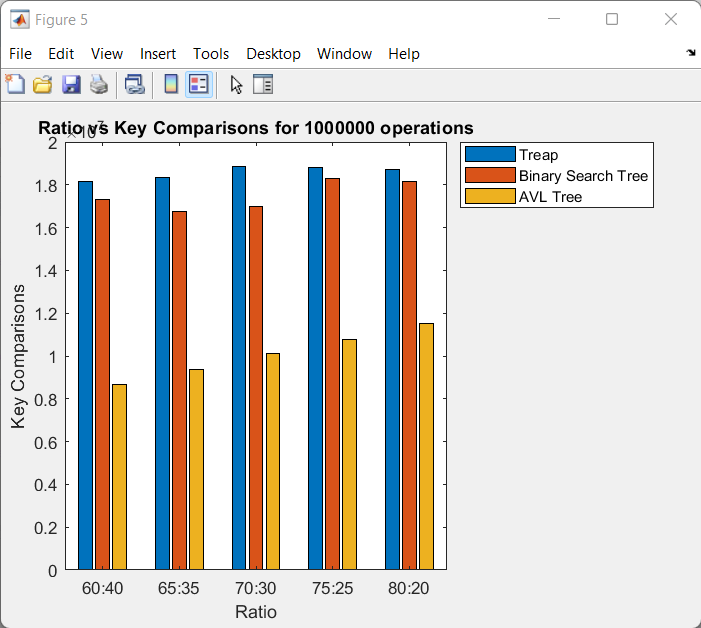
\includegraphics[scale=0.3]{key1M.png}
\end{center}
\subsubsection{Rotations}
\begin{center}
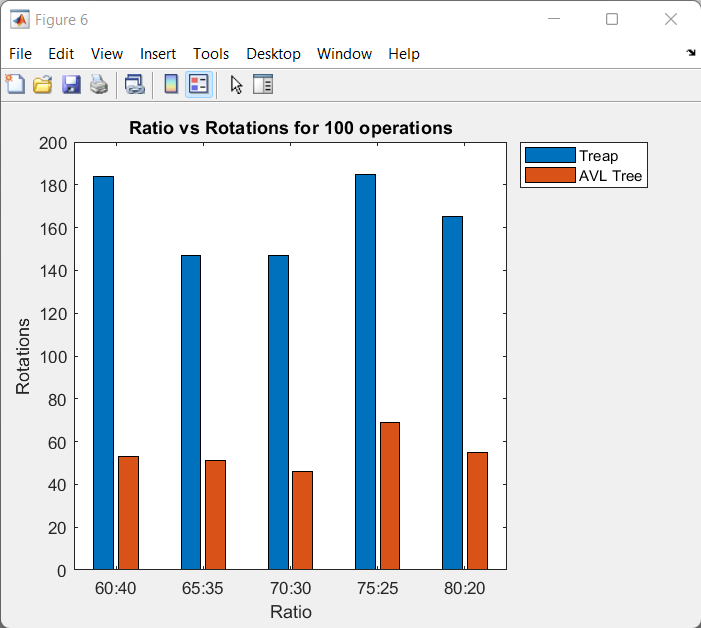
\includegraphics[scale=0.3]{rotations100.png}
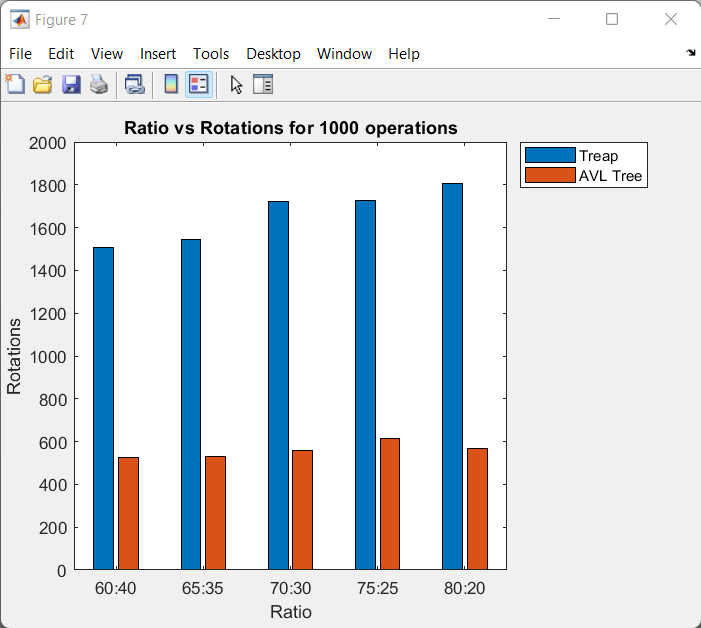
\includegraphics[scale=0.3]{rotations1K.png}
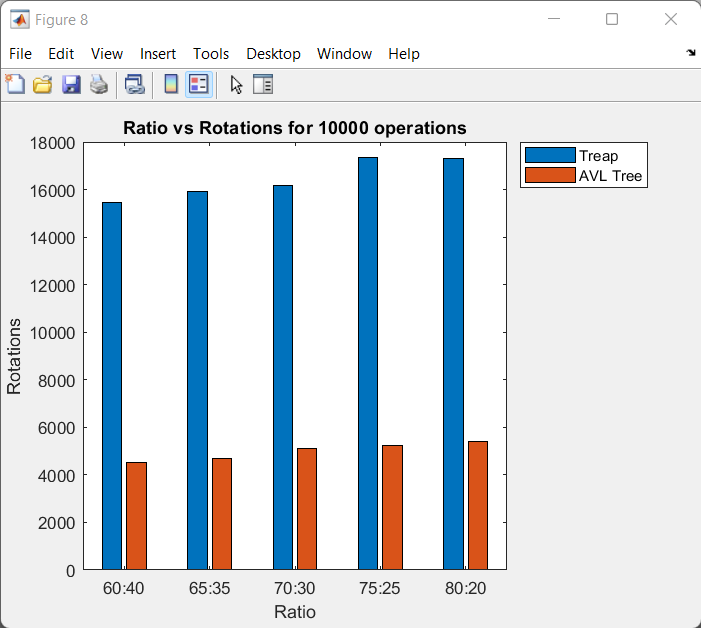
\includegraphics[scale=0.3]{rotations10K.png}
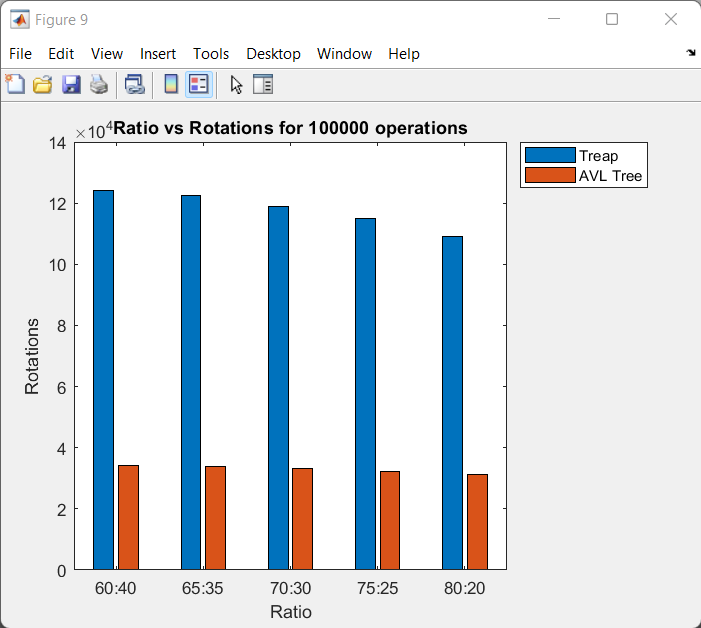
\includegraphics[scale=0.3]{rotations1L.png}
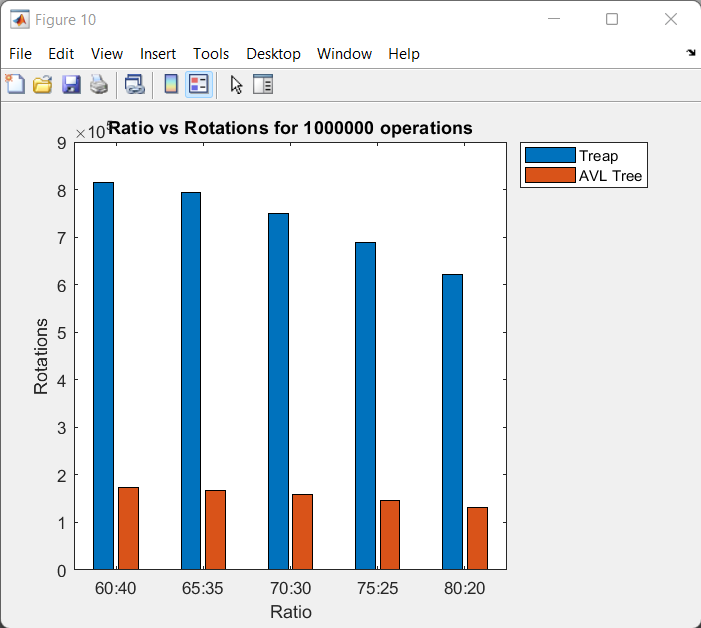
\includegraphics[scale=0.3]{rotations1M.png}
\end{center}
\subsubsection{Height of the tree}
\begin{center}
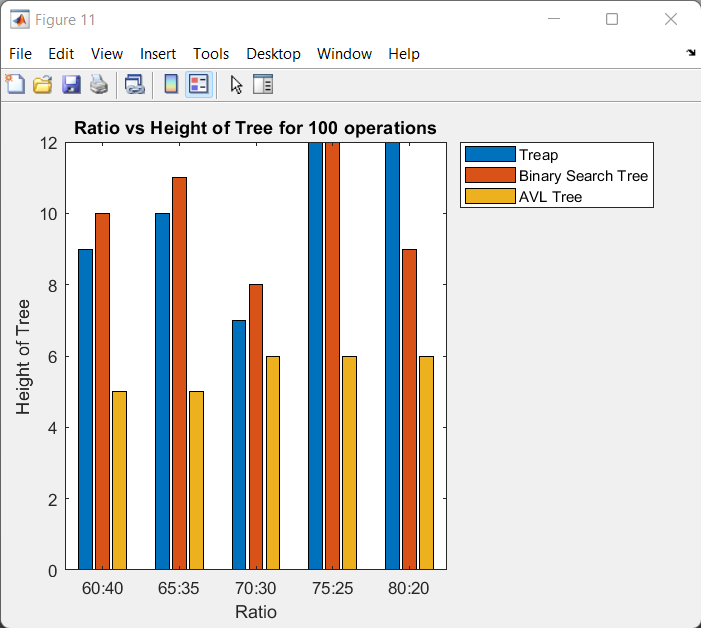
\includegraphics[scale=0.3]{height100.png}
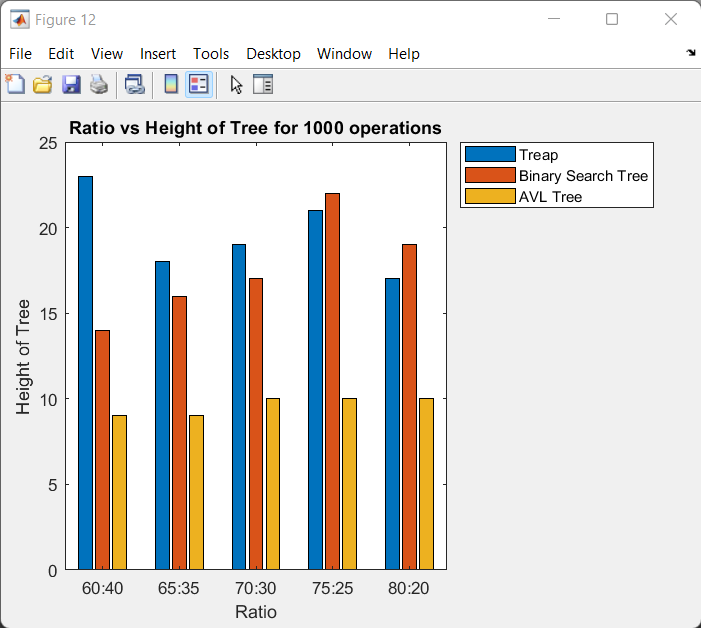
\includegraphics[scale=0.3]{height1K.png}
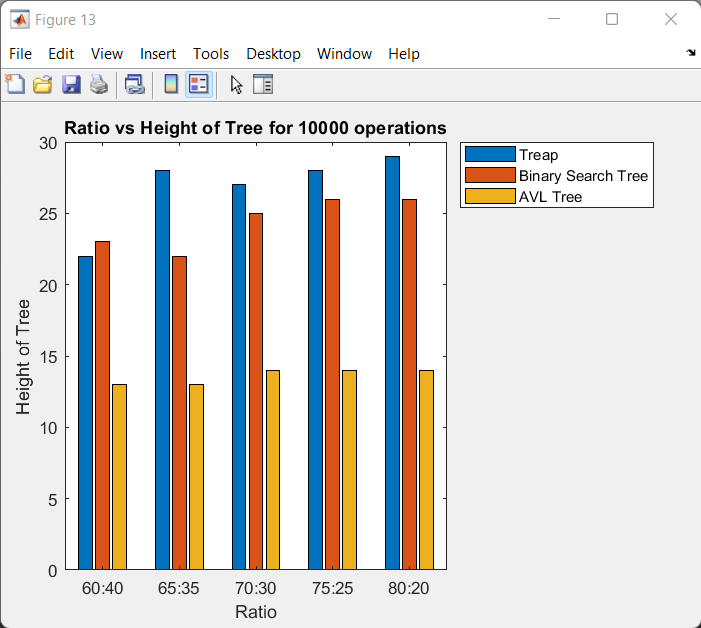
\includegraphics[scale=0.3]{height10K.png}
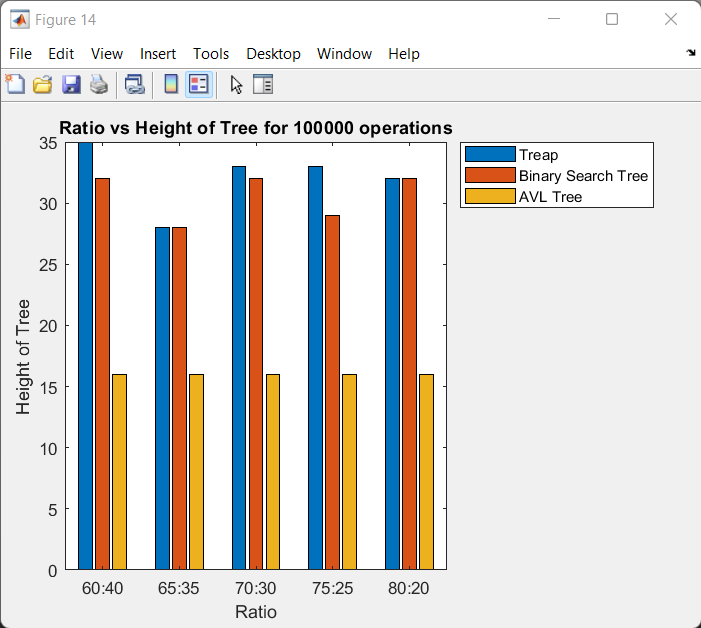
\includegraphics[scale=0.3]{height1L.png}
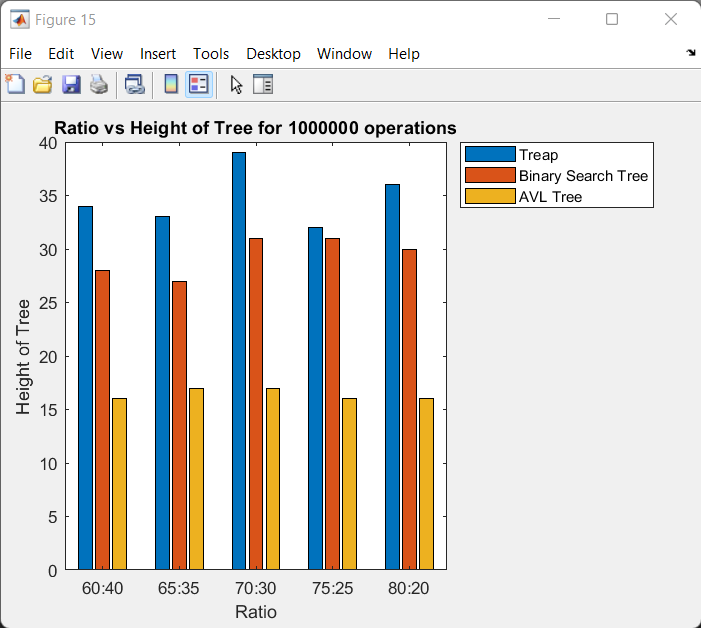
\includegraphics[scale=0.3]{height1M.png}
\end{center}
\subsubsection{Average Height of all nodes from root}
\begin{center}
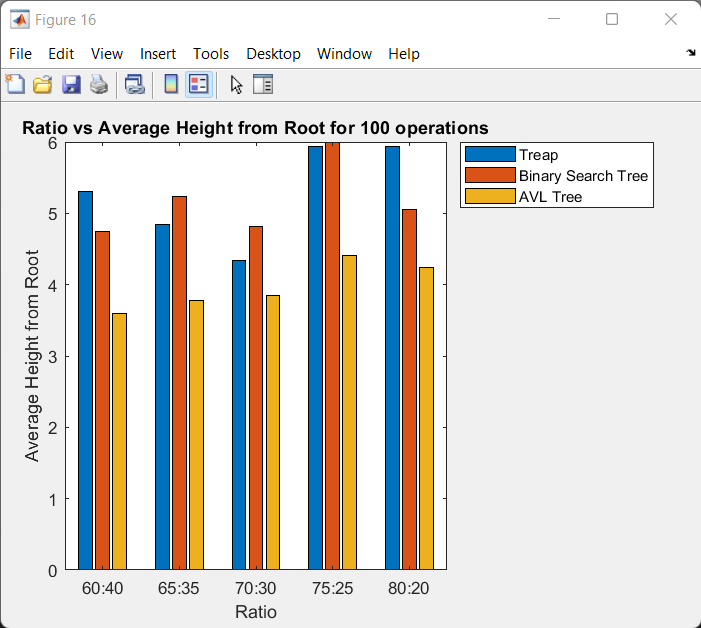
\includegraphics[scale=0.3]{root100.png}
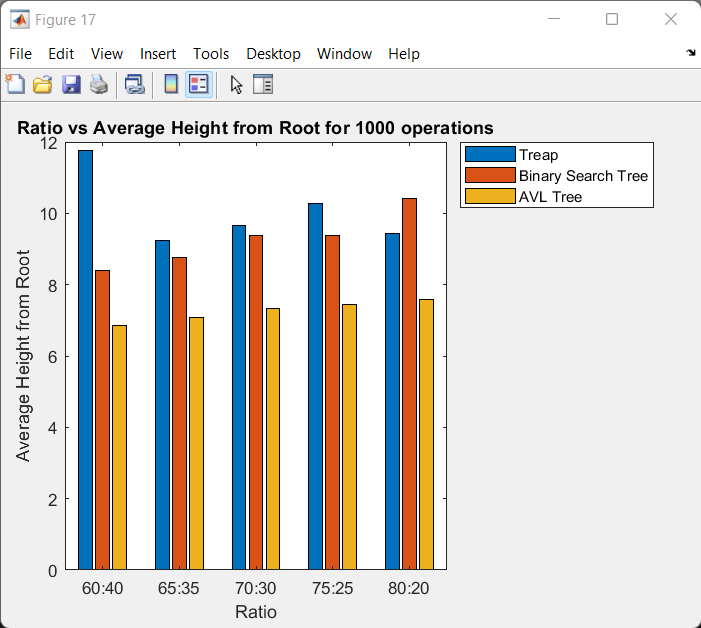
\includegraphics[scale=0.3]{root1K.png}
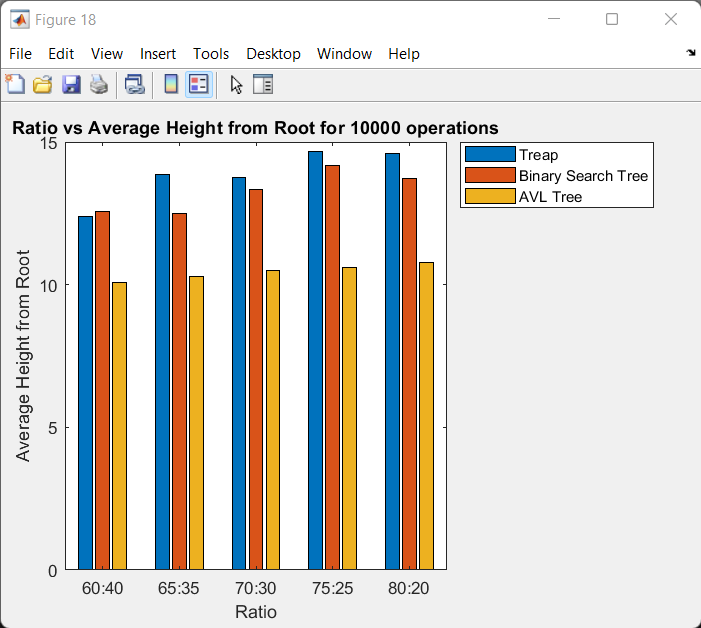
\includegraphics[scale=0.3]{root10K.png}
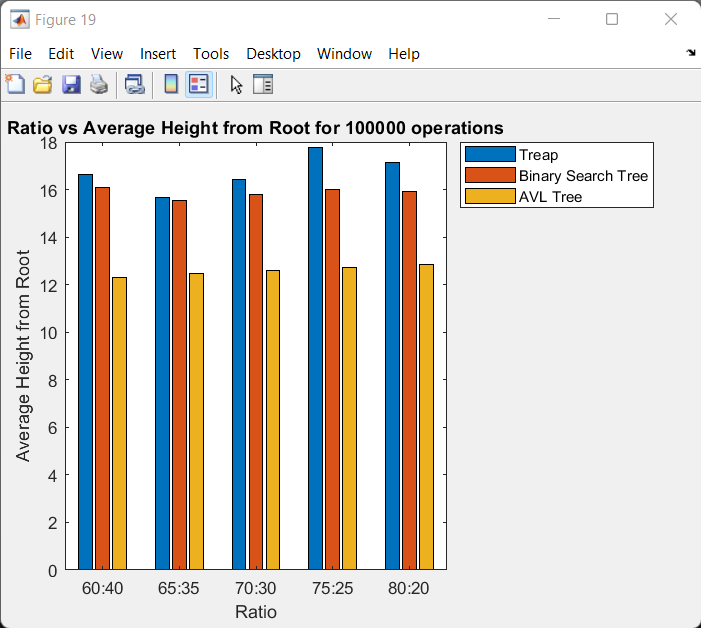
\includegraphics[scale=0.3]{root1L.png}
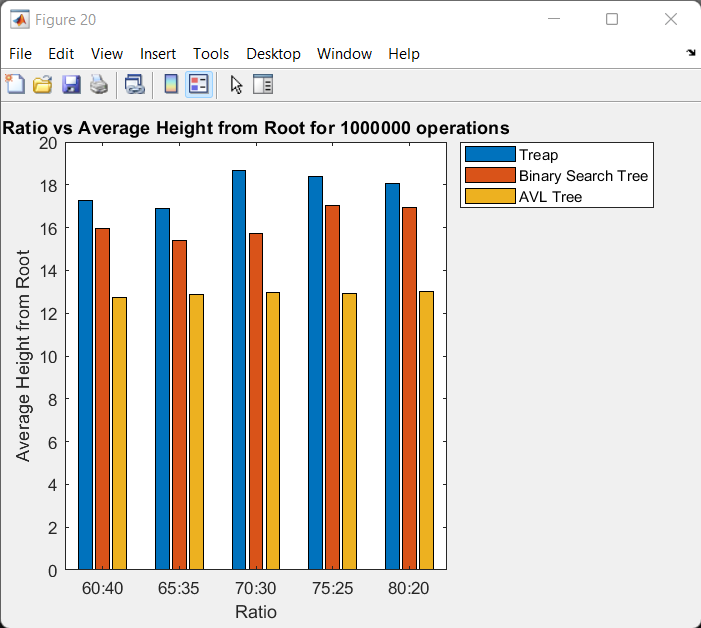
\includegraphics[scale=0.3]{root1M.png}
\end{center}
\subsubsection{Average Height of all nodes from bottom}
\begin{center}
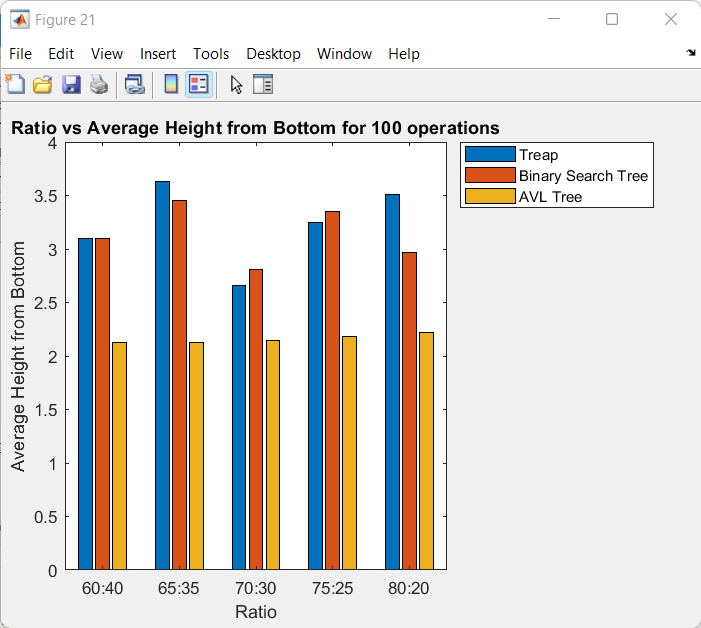
\includegraphics[scale=0.3]{bottom100.png}
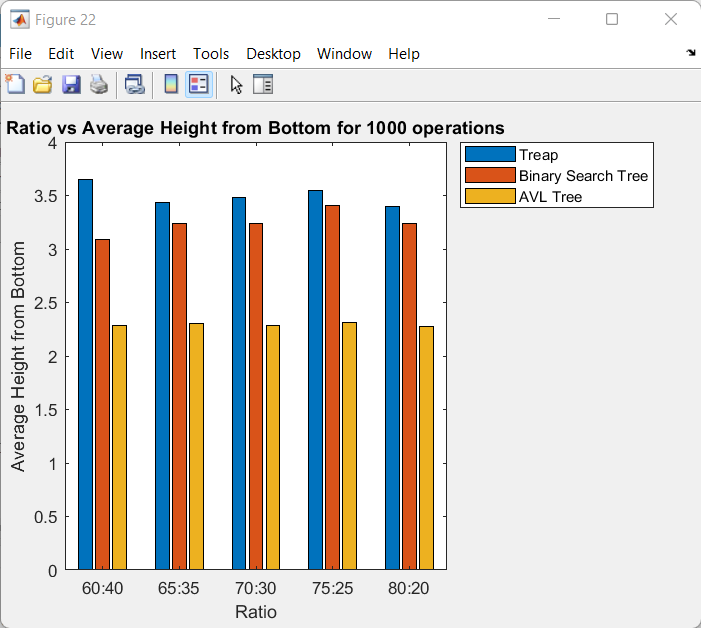
\includegraphics[scale=0.3]{bottom1K.png}
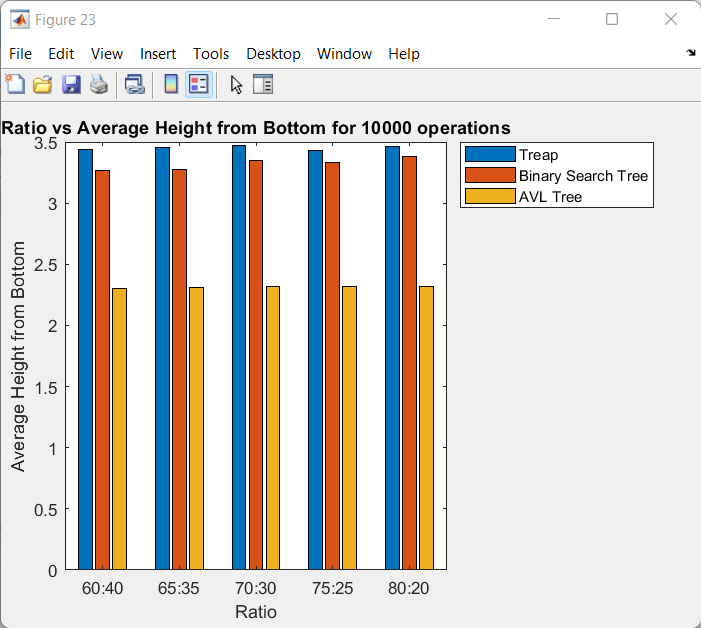
\includegraphics[scale=0.3]{bottom10K.png}
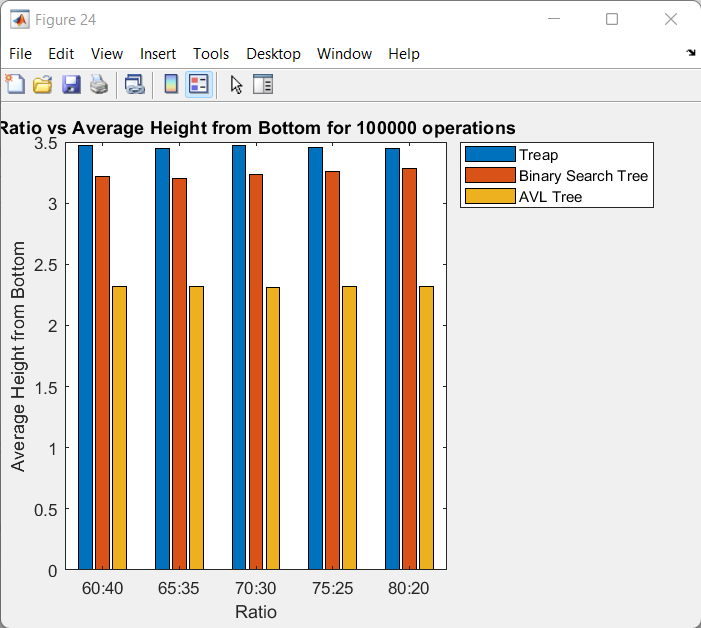
\includegraphics[scale=0.3]{bottom1L.png}
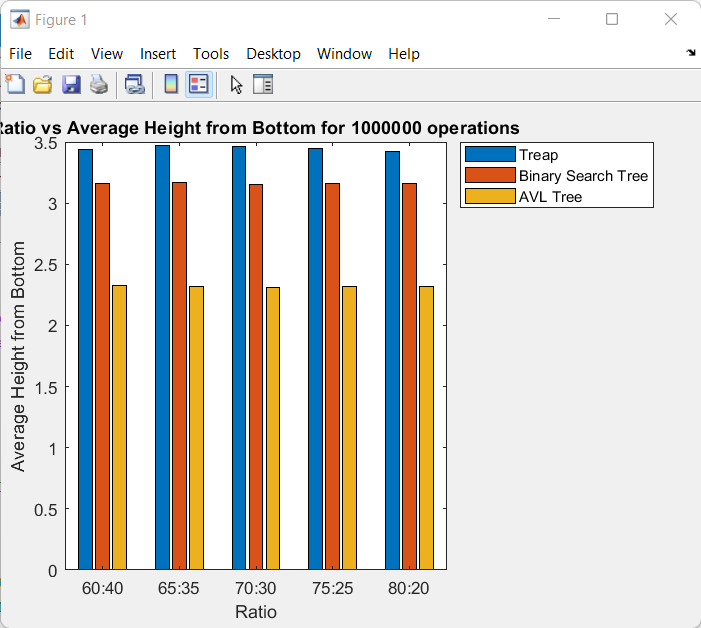
\includegraphics[scale=0.3]{bottom1M.png}
\end{center}
\subsubsection{Analysis and Catch}
AVL Tree clearly beats both treap and binary search tree. For most of the cases, we can observe a stability or a stable increse (or decrease) in case of AVL tree whereas the results for treap and binary search tree are not very stable. Also, AVL tree gives better performance in almost all types of parameters. As discussed, randomized search tree should perform better than binary search tree in most of the cases if we have a good random number generator in case of priority generation.\newline
But, here is a catch. Since in our experiment, we generated the key values randomly too, binary search tree is giving almost similar performance or somewhat better performance than randomized search tree, which might not happen in real world scenario if we have skewed or partially skewed key set. In that case binary search tree will give much worse results than randomized search tree. Let's have a look on that case.
\subsubsection{Worst case of BST which is not worst for RST}
After generating the final tree, all the key values are obtained from the treap and stored in a file. Then we sort the file and insert the keys to a new treap, a binary search tree and an AVL tree. The results are as follows.
\subsubsection{Parameters for $10000$ operations}
\begin{center}
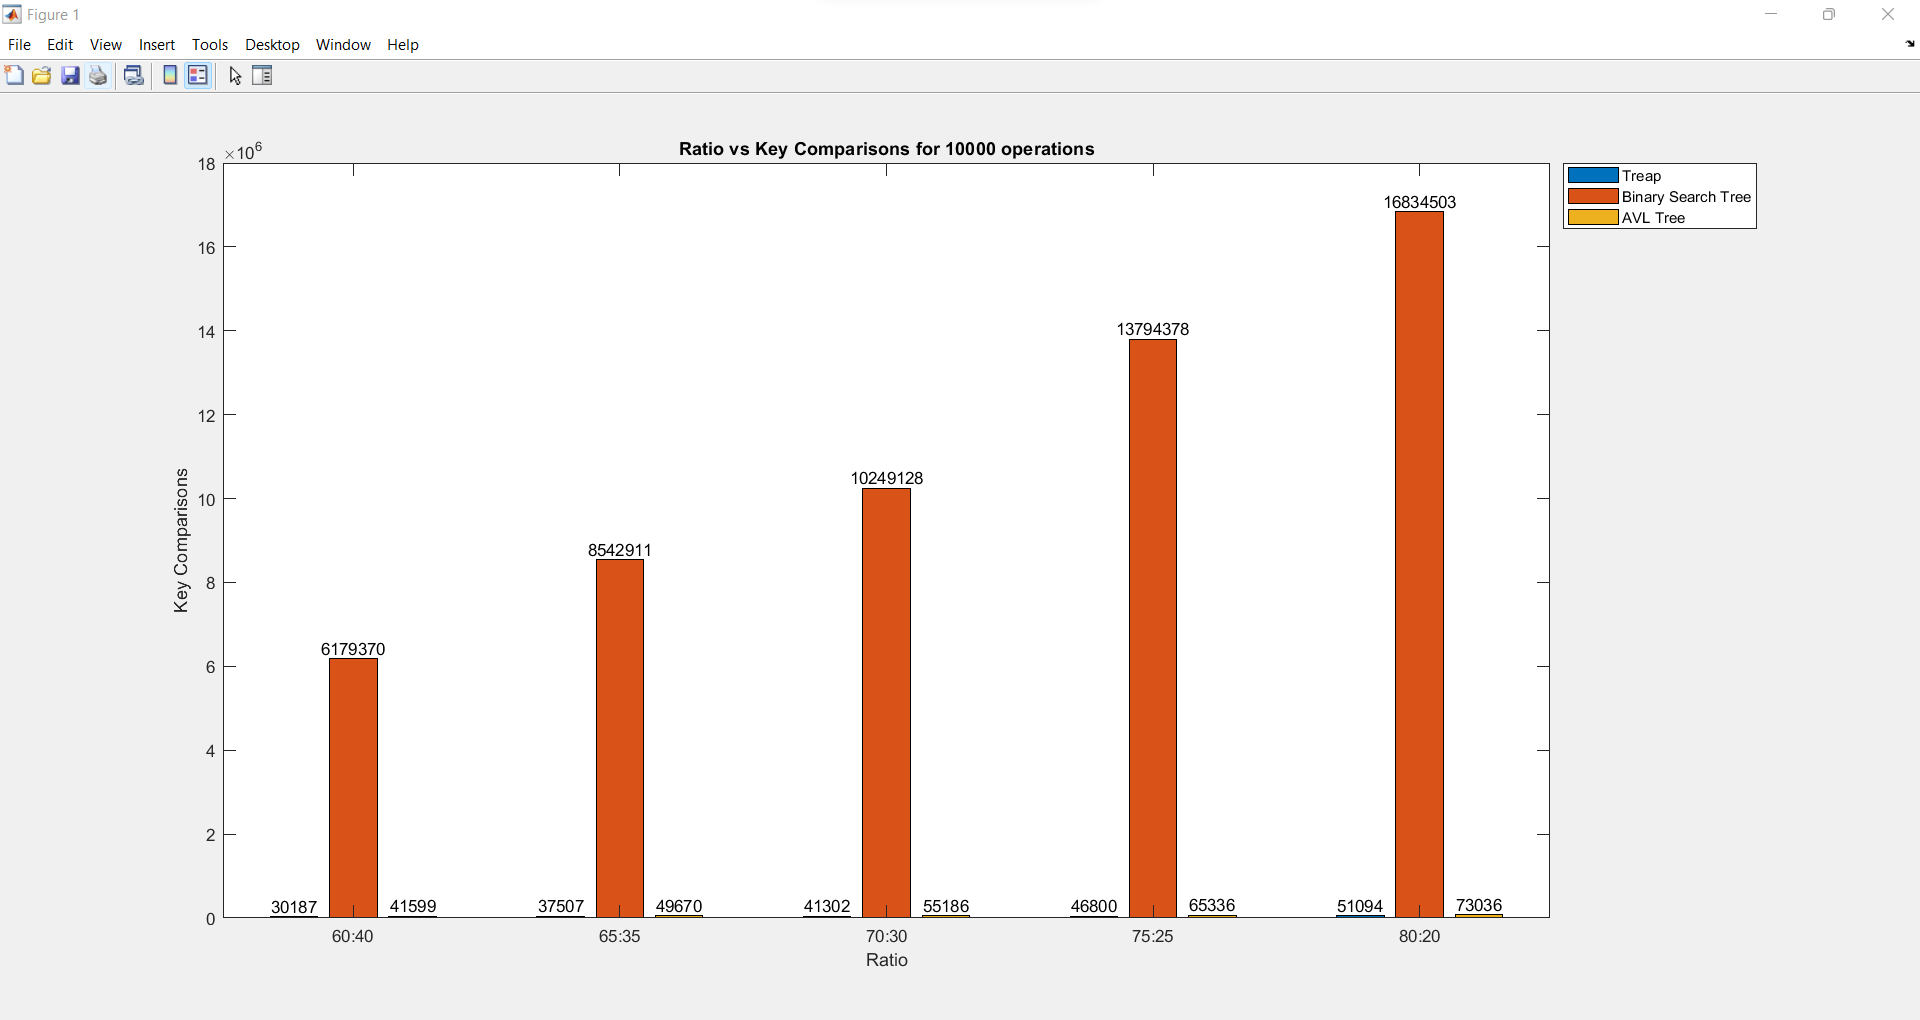
\includegraphics[scale=0.4]{wkey10K.png}
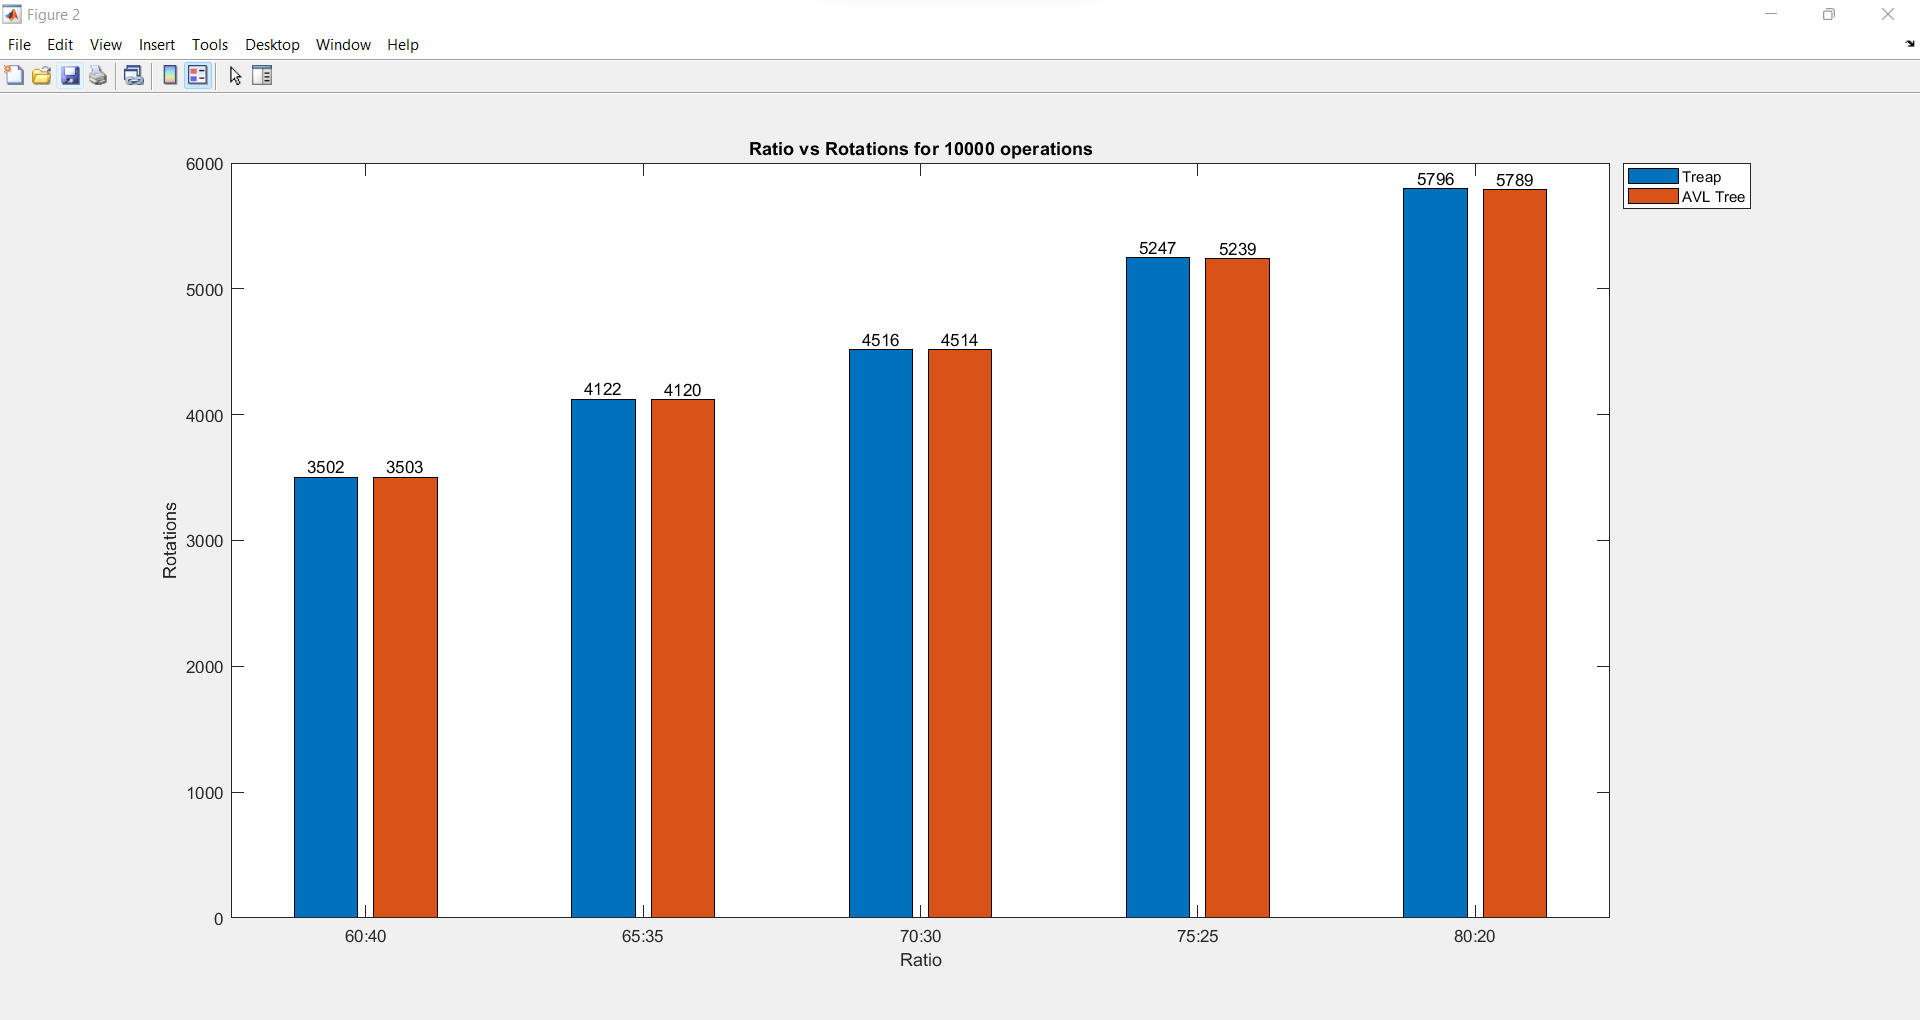
\includegraphics[scale=0.4]{wrotations10K.png}
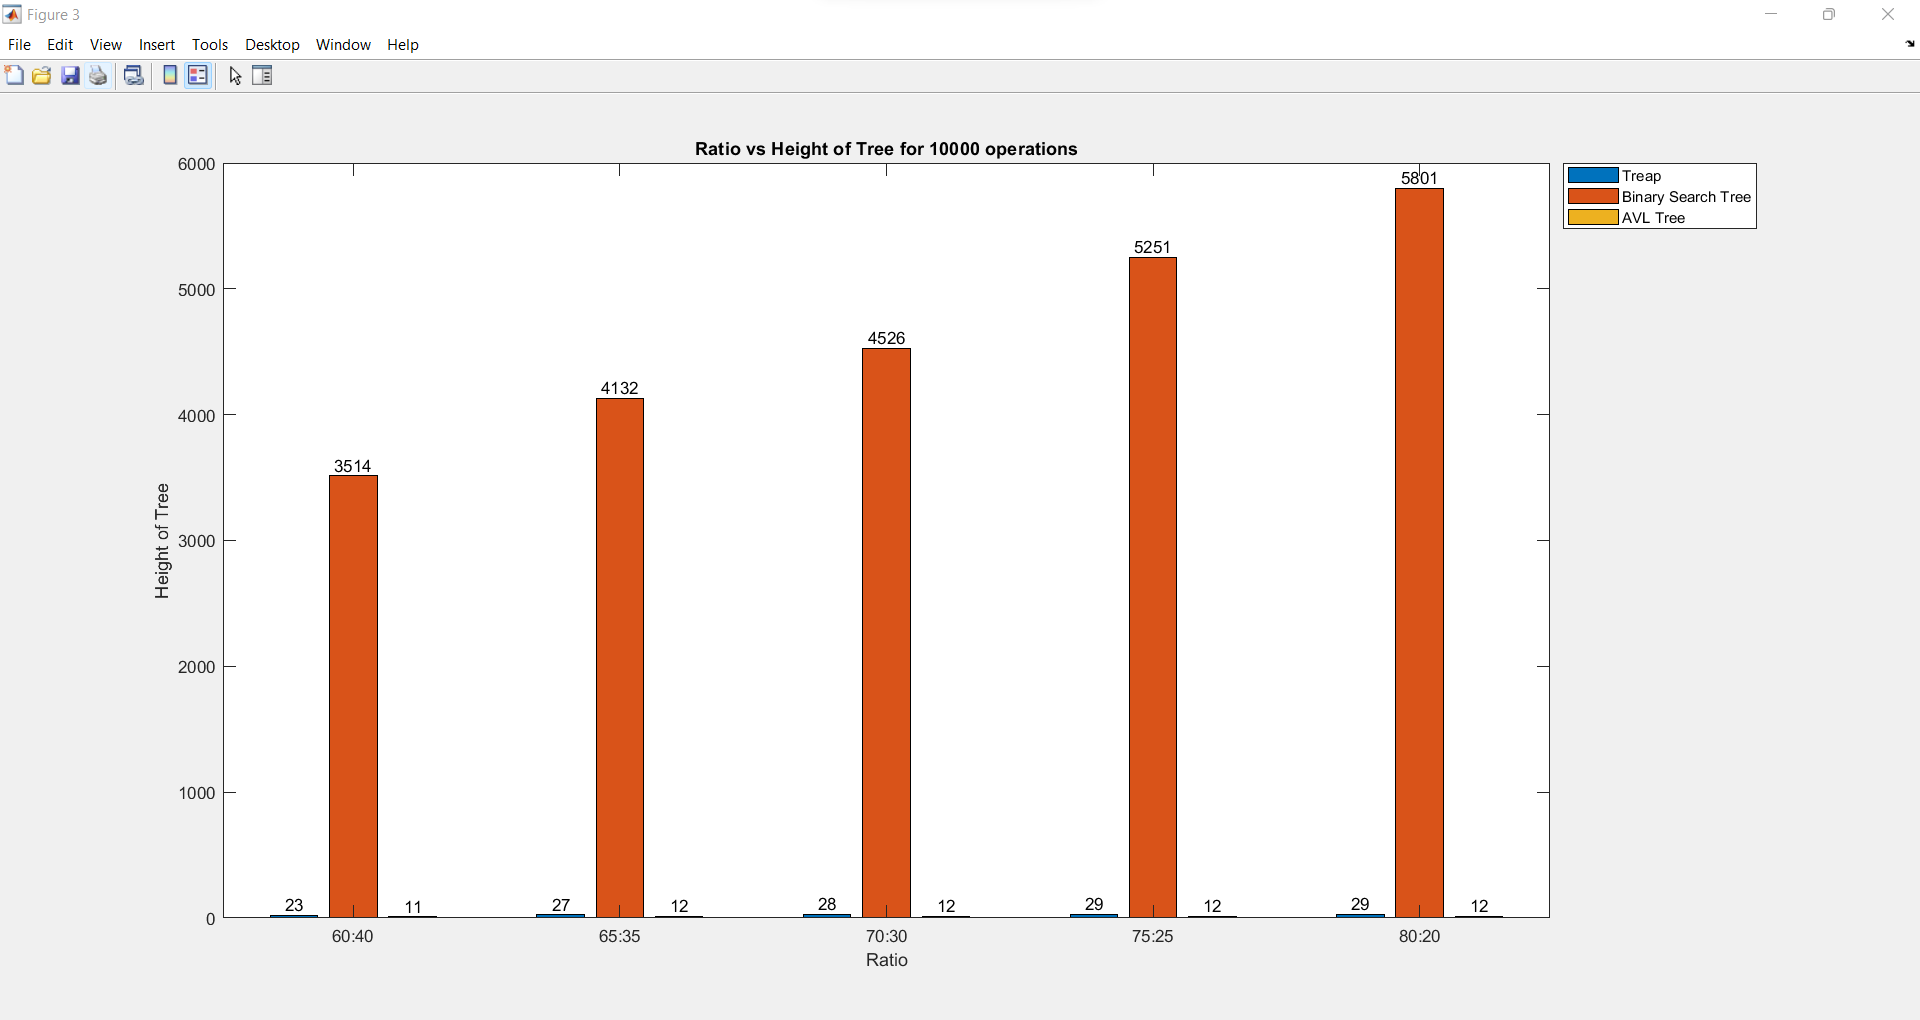
\includegraphics[scale=0.4]{wheight10K.png}
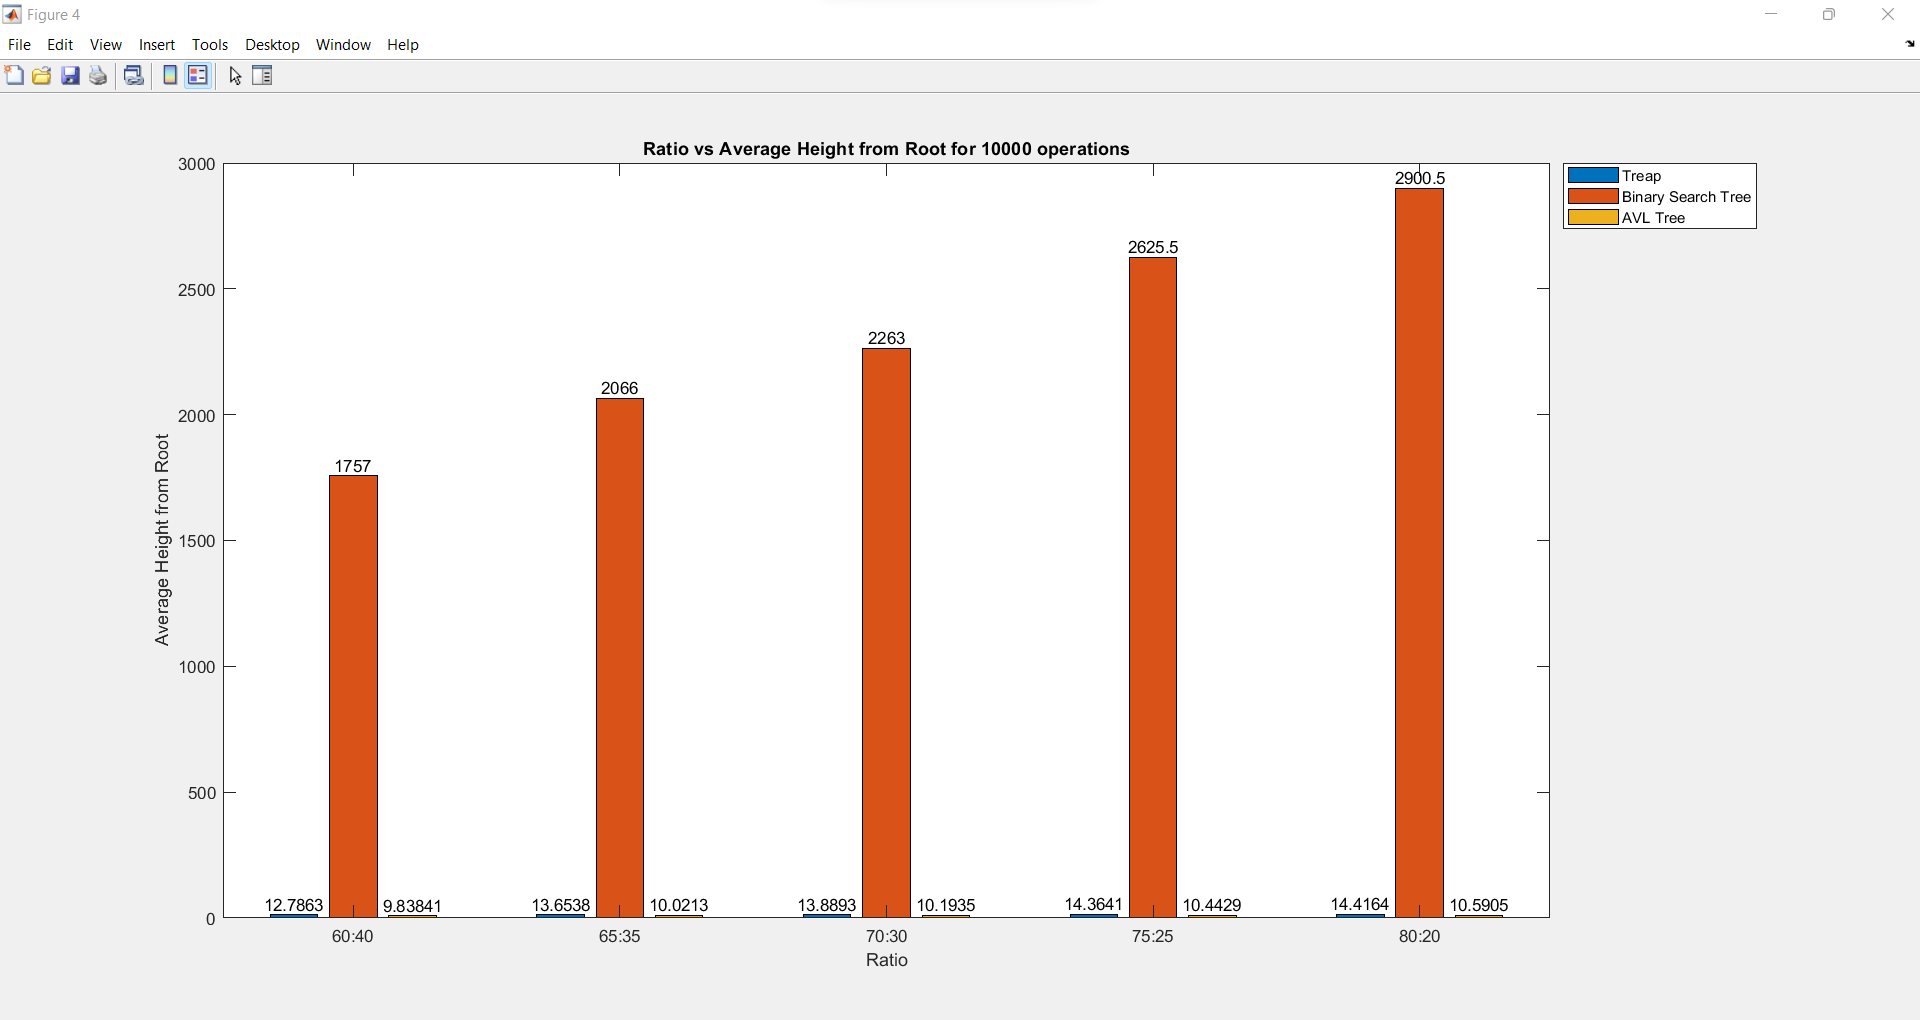
\includegraphics[scale=0.4]{wroot10K.png}
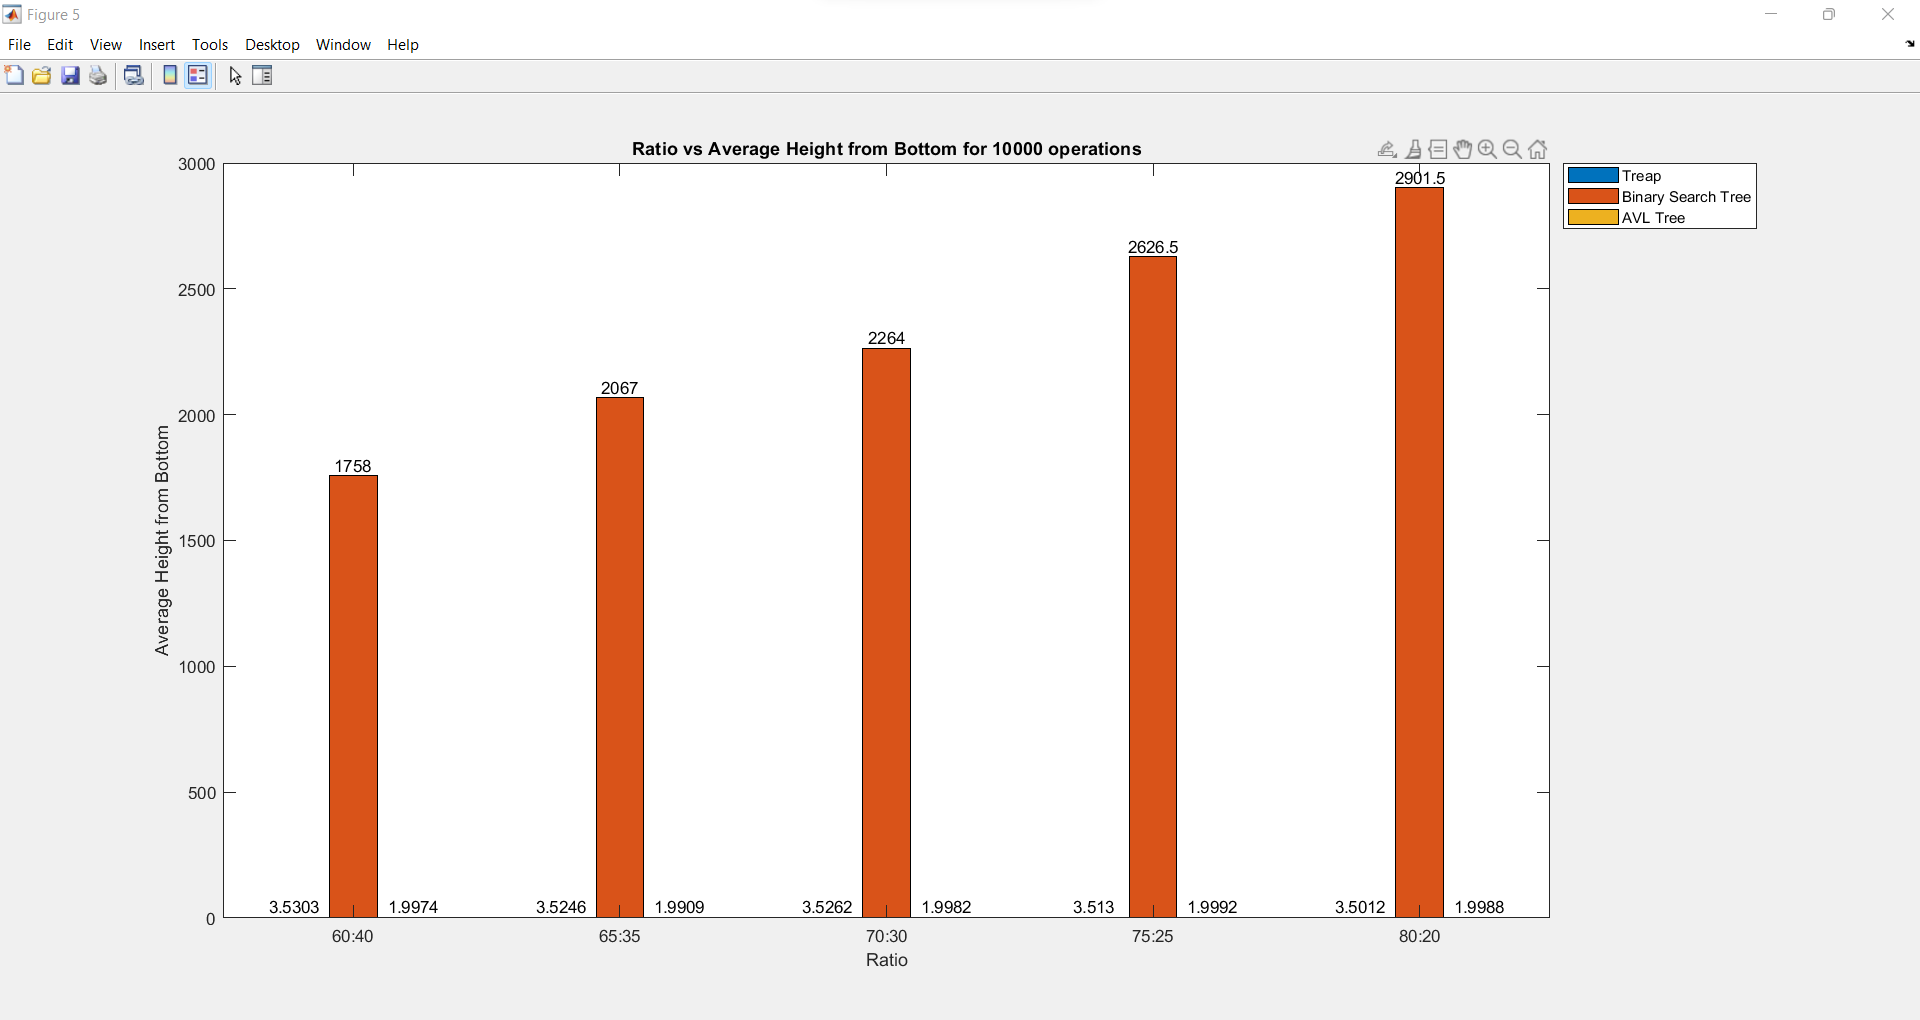
\includegraphics[scale=0.4]{wbottom10K.png}
\end{center}
The difference between binary search tree and randomized search tree is clearly visible. This was for the case of a completely skewed insertion key sequence. If the key set is not ccompletely random, it can be partially skewed. In that case also, binary search tree will give partially skewed performance whereas treap will give average case mostly.


\section{Comparison of Theoretical and Empirical results}
\subsection{Theoretical Claims}
\subsubsection{Worst case}
\begin{center}
\begin{tabular}{||p{4cm}||p{4cm}|p{3cm}|p{5cm}||}
\hline
& RST & BST & AVL Tree \\
\hline\hline
Key comparisons & $O(n\log n)\le$comp$\le O(n(n+1)/2)$ & $O(n(n+1)/2)$ & $O(n\log n)\le$comp$\le O(1.441*n\log n)$ \\ 
\hline
Rotations & insert$*O(h)+$delete$*O(h)$ & 0 & insert$*O(1)+$delete$*O(\log n)$;(or $O(1.441*\log n)$) \\
\hline
Height of tree & $O(\log n)\le$height$\le O(n)$ & $O(n)$ & $\le O(\log n)$ and $<O(1.441\log n)$ \\
\hline
Average height of nodes & $O(\log n)\le$height$\le O(n)$ & $O(n(n+1)/(2*n))$ & $\le O(\log n)$ and $<O(1.441\log n)$ \\
\hline
\end{tabular}
\end{center}

\subsection{Empirical results}
Let's consider one expected worst case performances for each of the trees. The tabulation will be as follows.
\subsubsection{$n=4591$}
File path : "/Experiments/7030/10000/10/9"
\begin{center}
\begin{tabular}{||c || c | c||} 
\hline
RST & Calculated from table & Actual \\
\hline\hline
Key comparisons & $4591*\log(4591)=55847\le$comp$\le 4591*4592/2=10540936$ & $150421$ \\
\hline
Rotations & $4591*28=128548$ & $16450$ \\
\hline
Height of tree & $12.16\le$height$<4591$ & $28$ \\
\hline
Average height of nodes & $12\le$height$<4591$ & $15.3143$ \\
\hline
\end{tabular}
\end{center}
\subsubsection{$n=4527$}
File path : "/Worst case keys/evaluation10K70.txt"
\begin{center}
\begin{tabular}{||c || c | c||} 
\hline
BST & Calculated from table & Actual \\
\hline\hline
Key comparisons & $4527*4528/2=10249128$ & $10249128$ \\ 
\hline
Rotations & $0$ & $0$ \\
\hline
Height of tree & $4526$ & $4526$ \\
\hline
Average height of nodes & $(4526*4527)/(2*4527)=2263$ & $2263$ \\
\hline
\end{tabular}
\end{center}
\subsubsection{$n=5252$}
File path : "/Worst case keys/evaluation10K75.txt"
\begin{center}
\begin{tabular}{||c || c | c||} 
\hline
AVL Tree & Calculated from table & Actual \\
\hline\hline
Key comparisons & $\le 5252*\log(5252)=64908$ and $<1.441*64908=93532$ & $65336$ \\ 
\hline
Rotations & $5252*1=5252$ & $5239$ \\
\hline
Height of tree & $\le 12.36$ and $<1.441*12.36=17.81$ & $12$ \\
\hline
Average height of nodes & $\le 12.36$ and $<1.441*12.36=17.81$ & $10.4429$ \\
\hline
\end{tabular}
\end{center}
We can see, empirical results are very similar to theoretical results.

\end{document}